%%%%%%%%%%%%%%%%%%%%%%%%%%%%%%%%%%%%%%%%%
% Short Sectioned Assignment
% LaTeX Template
% Version 1.0 (5/5/12)
%
% This template has been downloaded from:
% http://www.LaTeXTemplates.com
%
% Original author:
% Frits Wenneker (http://www.howtotex.com)
%
% License:
% CC BY-NC-SA 3.0 (http://creativecommons.org/licenses/by-nc-sa/3.0/)
%
%%%%%%%%%%%%%%%%%%%%%%%%%%%%%%%%%%%%%%%%%

%----------------------------------------------------------------------------------------
%	PACKAGES AND OTHER DOCUMENT CONFIGURATIONS
%----------------------------------------------------------------------------------------

\documentclass[paper=a4, fontsize=11pt]{scrartcl} % A4 paper and 11pt font size

\usepackage[T1]{fontenc} % Use 8-bit encoding that has 256 glyphs
\usepackage{fourier} % Use the Adobe Utopia font for the document - comment this line to return to the LaTeX default
\usepackage[english]{babel} % English language/hyphenation
\usepackage{amsmath,amsfonts,amsthm} % Math packages

\usepackage{graphicx}
\usepackage{float}

\usepackage{sectsty} % Allows customizing section commands
\allsectionsfont{\normalfont\scshape} % Make all sections centered, the default font and small caps

\usepackage{fancyhdr} % Custom headers and footers
\pagestyle{fancyplain} % Makes all pages in the document conform to the custom headers and footers
\fancyhead{} % No page header - if you want one, create it in the same way as the footers below
\fancyfoot[L]{} % Empty left footer
\fancyfoot[C]{} % Empty center footer
\fancyfoot[R]{\thepage} % Page numbering for right footer
\renewcommand{\headrulewidth}{0pt} % Remove header underlines
\renewcommand{\footrulewidth}{0pt} % Remove footer underlines
\setlength{\headheight}{13.6pt} % Customize the height of the header

\numberwithin{equation}{section} % Number equations within sections (i.e. 1.1, 1.2, 2.1, 2.2 instead of 1, 2, 3, 4)
\numberwithin{figure}{section} % Number figures within sections (i.e. 1.1, 1.2, 2.1, 2.2 instead of 1, 2, 3, 4)
\numberwithin{table}{section} % Number tables within sections (i.e. 1.1, 1.2, 2.1, 2.2 instead of 1, 2, 3, 4)

\setlength\parindent{0pt} % Removes all indentation from paragraphs - comment this line for an assignment with lots of text

%----------------------------------------------------------------------------------------
%	TITLE SECTION
%----------------------------------------------------------------------------------------

\newcommand{\horrule}[1]{\rule{\linewidth}{#1}} % Create horizontal rule command with 1 argument of height

\title{	
\normalfont \normalsize 
\textsc{BRSU} \\ [25pt] % Your university, school and/or department name(s)
\horrule{0.5pt} \\[0.4cm] % Thin top horizontal rule
\huge Homework for Artificial Intelligence for Robotics\\Assignment 8 \\ % The assignment title
\horrule{2pt} \\[0.5cm] % Thick bottom horizontal rule
}

\author{Bastian Lang} % Your name

\date{\normalsize\today} % Today's date or a custom date

\begin{document}

\maketitle % Print the title

\section{Practical Part}

\subsection{Task}
\textit{Solve the same Travelling Salesman Problem as the previous assignment, but using Simulated Annealing and all cities in the file. Get the best solution for different computation
time (say 5, 10, 15 minutes).}

\subsection{Approach}
For this task I reused classes from the previous travelling salesman assignment to represent cities and solutions and to read the cities from the file. But I used another approach for the hill climbing algorithm. Instead of first computing every possible successor state and only then decide on the best one, I now create only one random successor state by swapping two cities and decide right away on sticking with it or dropping it.

As a temperature I chose the remaining runtime of the algorithm. Initially the user can give a runtime (in minutes). The longer the algorithm runs, the smaller the temperature gets. If it becomes zero the algorithm stops. 

For the probability to choose a worse successor I included a constant into the formula similar to the boltzmann constant, which is roughly $8.6 * 10^{-5}$ (I choose $10^{-6}$. 

I executed the program for 5 min, 10 min, 15 minutes and 30 minutes. The results can be seen below.

\subsection{Results}

\subsubsection{5 min}

\begin{figure}[h]
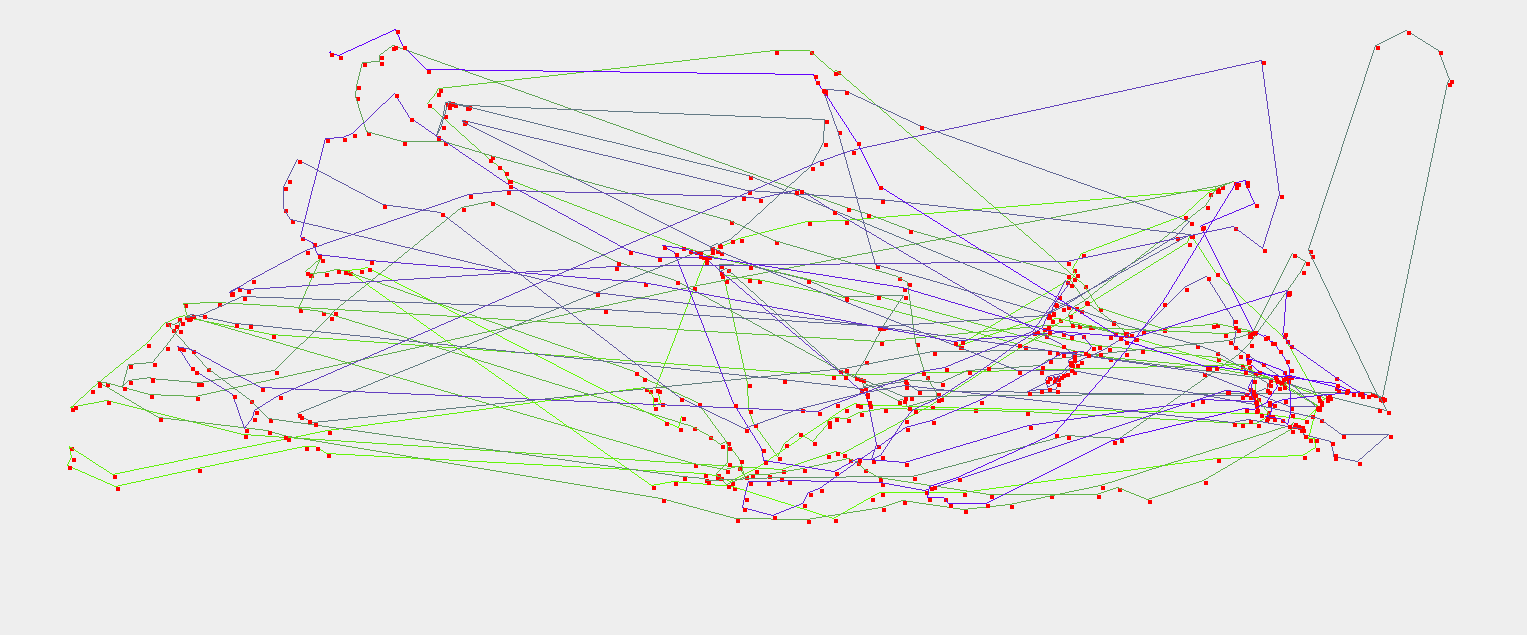
\includegraphics[width=\textwidth]{5min.png}
\caption{path after 5 minutes computation}
\label{tenMin}
\end{figure}

Path length: 9012.441310

Number of iterations: 2798073

0.061399 percent of total iterations chose a worse successor

\subsubsection{10 min}

\begin{figure}[h]
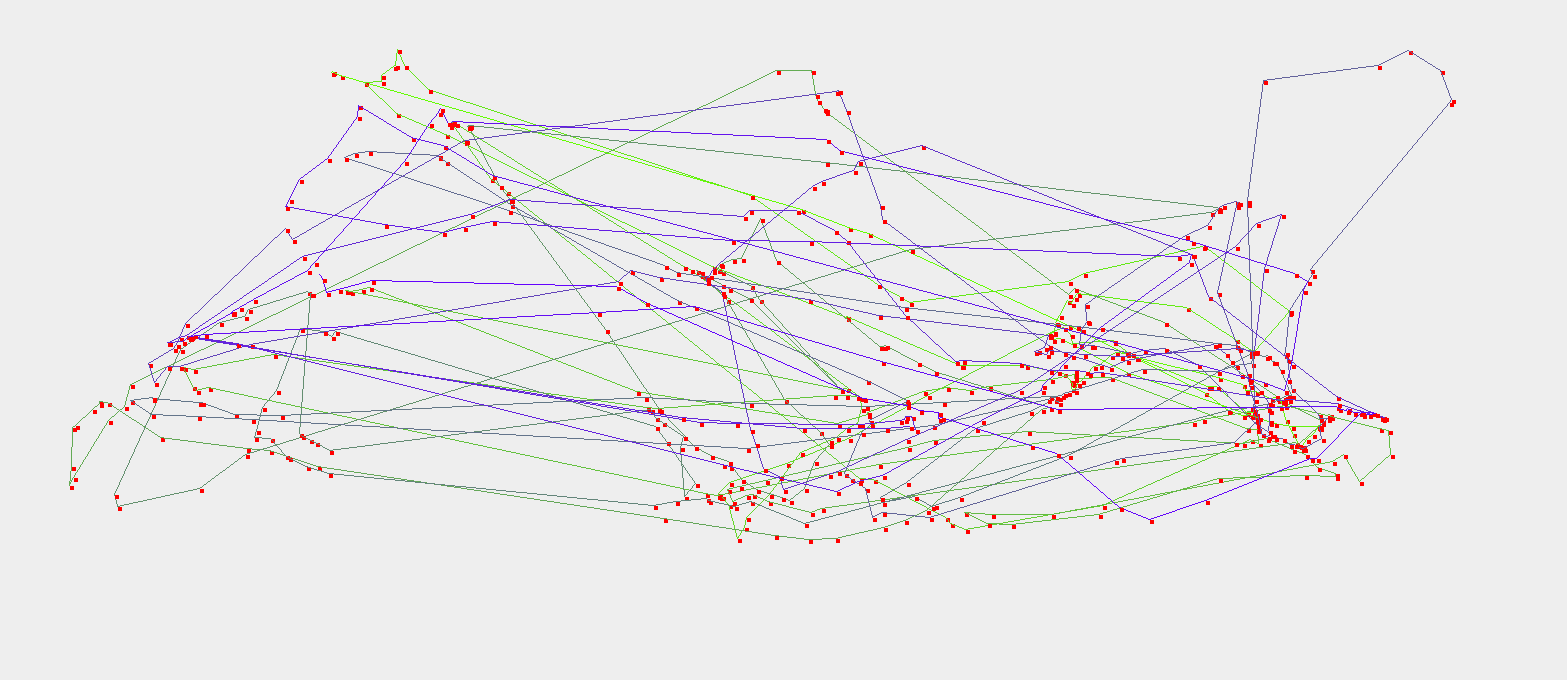
\includegraphics[width=\textwidth]{10min.png}
\caption{path after 10 minutes computation}
\label{tenMin}
\end{figure}

Path length: 8194.656366

Number of iterations: 5587871

0.092987 percent of total iterations chose a worse successor

\subsubsection{15 min}

\begin{figure}[h]
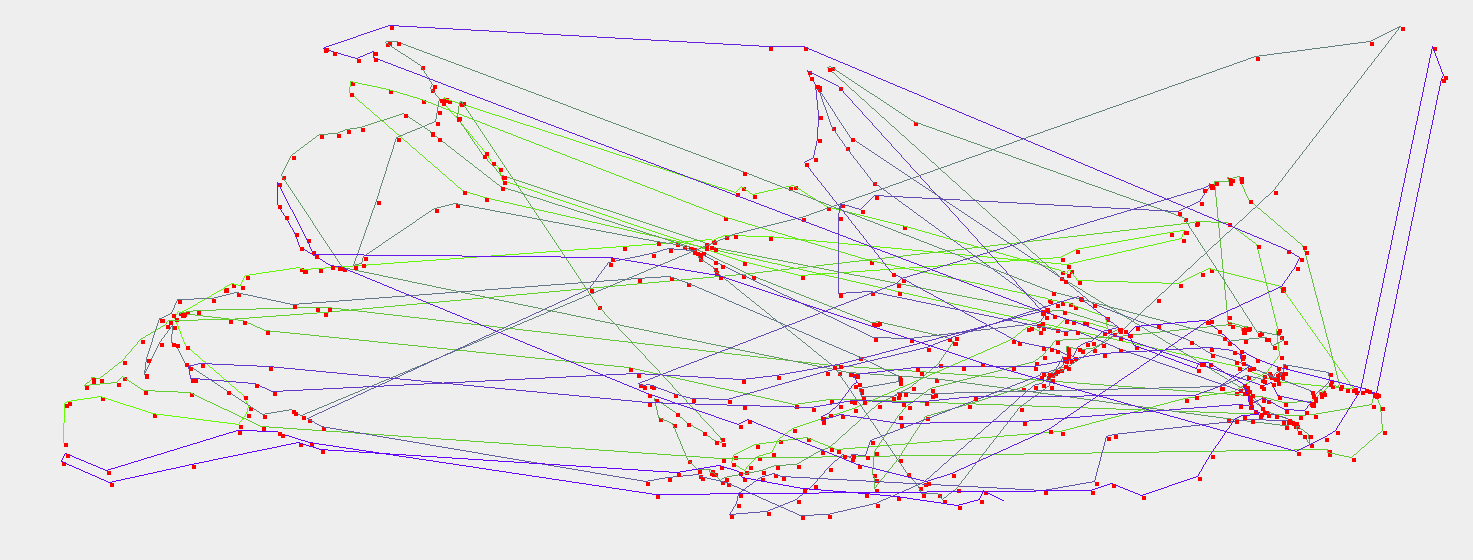
\includegraphics[width=\textwidth]{15min.png}
\caption{path after 15 minutes computation}
\label{tenMin}
\end{figure}

Path length: 7959.778290

Number of iterations: 8363361

0.127281 percent of total iterations chose a worse successor

\subsubsection{30 min}

\begin{figure}[h]
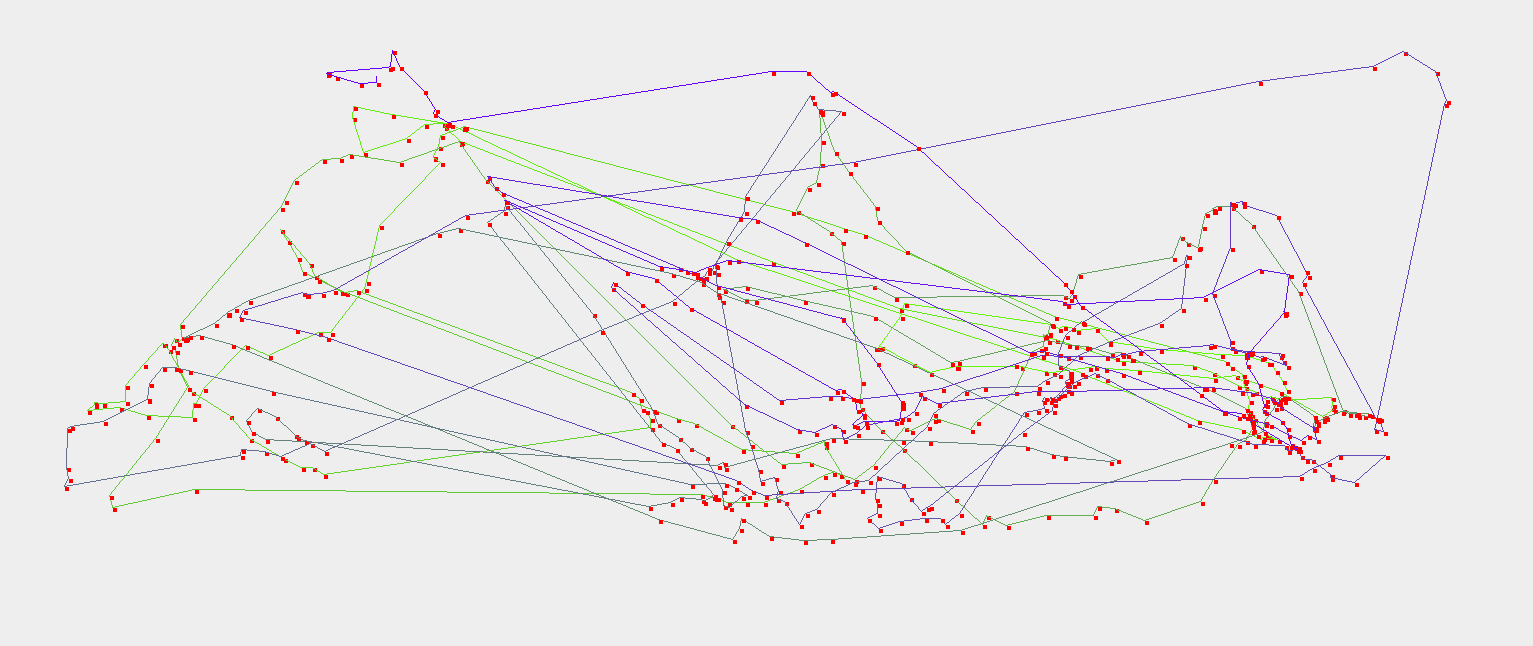
\includegraphics[width=\textwidth]{30min.png}
\caption{path after 30 minutes computation}
\label{tenMin}
\end{figure}

Path length: 5677.814568

Number of iterations: 16751338

0.196319 percent of total iterations chose a worse successor


\section{Theoretical Part}
\subsection{Task}
Consider the following puzzle and represent it as a Constrain Satisfaction Problem. Do
not solve/implement it. Provide only the variables, the values of those variables, and the
constraints.
\begin{itemize}
\item There are five houses.
\item The Englishman lives in the red house.
\item The Spaniard owns the dog.
\item Coffee is drunk in the green house.
\item The Ukrainian drinks tea.
\item The green house is immediately to the right of the ivory house.
\item The Old Gold smoker owns snails.
\item Kools are smoked in the yellow house.
\item Milk is drunk in the middle house.
\item The Norwegian lives in the first house.
\item The man who smokes Chesterfields lives in the house next to the man with the fox.
\item Kools are smoked in a house next to the house where the horse is kept.
\item The Lucky Strike smoker drinks orange juice.
\item The Japanese smokes Parliaments.
\item The Norwegian lives next to the blue house.
\end{itemize}
The question posed by the puzzle is: Who drinks water? Who owns the zebra?

\subsection{Solution}
A \textbf{Constraint Satisfaction Problem} is described by defining the \textbf{possible states} and the \textbf{goal test}. The state consists of \textbf{variables} and their \textbf{domains}. The goal test consists of all combinations of value assignments to variables that have to be fulfilled for a state to be considered a solution to the problem.
\subsubsection{Variables}
The Variables are the five houses:\\
Variables = \{First, Second, Third, Fourth, Fifth \}
\subsubsection{Variable Domains}
Each variable consists of exactly five values: The color of the house, the person living in the house, the pet of the person living in the house, the drink the person in the house drinks and the brand of the smoke the person in the house smokes.\\\\
Domain = \{\\
\{red, green, ivory, yellow, blue\},\\
\{Englishman, Spaniard, Ukrainian, Norwegian, Japanese\},\\
\{tea, coffee, milk, orange juice, water\},\\
\{dog, horse, snails, fox, zebra\},\\
\{Lucky Strike, Parliaments, Kools, Old Gold, Chesterfield\}\\
\}.

\subsubsection{Goal Test}
Assume that each house has an index according to it's place (First = 1, Second = 2, Third = 3, Fourth = 4 and Fifth = 5) and that \textit{index\{...\}} returns the house's index of a given value, then the constraints are the following:
\begin{itemize}
\item index\{Englishman\} == index\{red\}
\item index\{Spaniard\} == index\{dog\}
\item index\{coffee\} == index\{green\}
\item index\{Ukrainian\} == index\{tea\}
\item index\{green\} == index\{ivory -1\}
\item index\{Old Gold\} == index\{snails\}
\item index\{Kools\} == index\{yellow\}
\item index\{milk\} == 3
\item index\{Norwegian\} == 1
\item index\{Chesterfield\} == index\{fox\} + 1 $\vert\vert$ index\{Chesterfield\} == index\{fox\} - 1
\item index\{Kools\} == index\{horse\} + 1 $\vert\vert$ index\{Kools\} == index\{horse\} - 1
\item index\{Lucky Strike\} == index\{orange juice\}
\item index\{Japanese\} == index\{Parliament\}
\item index\{Norwegian\} == index\{blue\} + 1 $\vert\vert$ index\{Norwegian\} == index\{blue\} - 1
\end{itemize}

\section{Practical Part}

\subsection{Task}
Solve the same Travelling Salesman Problem as the previous assignment, but using Sim-
ulated Annealing and all cities in the file. Get the best solution for different computation
time (say 5, 10, 15 minutes).

\subsection{Approach}

\subsection{Result}




\end{document}